% Adapted from the author's public Erdos Paper IV v1.23 series_template.tex.
% Layout provenance is recorded in 02_validation; the Markdown is semantic authority.
\documentclass[spanish,11pt,a4paper]{article}
\usepackage[margin=1in]{geometry}
\usepackage{fontspec}
\setmainfont{lmroman10-regular.otf}[BoldFont=lmroman10-bold.otf,ItalicFont=lmroman10-italic.otf,BoldItalicFont=lmroman10-bolditalic.otf]
\setsansfont{lmsans10-regular.otf}[BoldFont=lmsans10-bold.otf]
\setmonofont{lmmono10-regular.otf}[Scale=MatchLowercase]
\usepackage{amsmath,amssymb}
\providecommand{\mathscr}{\mathcal}
\usepackage[spanish,es-noshorthands,es-tabla]{babel}
\usepackage{microtype,parskip}
\usepackage{longtable,booktabs,array,calc}
\usepackage{xcolor,xurl}
\usepackage{hyperref,bookmark}
\usepackage{etoolbox,needspace}
\setcounter{secnumdepth}{-\maxdimen}
\setlength{\emergencystretch}{3em}
\providecommand{\tightlist}{\setlength{\itemsep}{0pt}\setlength{\parskip}{0pt}}
\newcounter{none}
\AtBeginEnvironment{longtable}{\Needspace{8\baselineskip}\small}
\pretocmd{\section}{\Needspace{5\baselineskip}}{}{}
\pretocmd{\subsection}{\Needspace{4\baselineskip}}{}{}
\pretocmd{\subsubsection}{\Needspace{4\baselineskip}}{}{}
\urlstyle{same}

\usepackage{graphicx}
\providecommand{\pandocbounded}[1]{#1}
\hypersetup{pdftitle={El espectro exacto de tipos de bloque en el problema de Colbourn–Dinitz–Rosa},pdfauthor={Juan Pablo Traverso Gianini},pdflang={es},colorlinks=true,linkcolor=blue,urlcolor=blue}
\title{El espectro exacto de tipos de bloque en el problema de Colbourn–Dinitz–Rosa}
\author{Juan Pablo Traverso Gianini\\\small Investigador independiente, Santiago, Chile\\\small \href{mailto:jtraverso@gmail.com}{jtraverso@gmail.com}\\\small \href{https://orcid.org/0009-0003-6068-4096}{ORCID: 0009-0003-6068-4096}}
\date{}
\begin{document}
\raggedbottom
\maketitle
\textbf{Artículo I. Bicoloraciones de sistemas triples de Steiner.}\\\textbf{Preprint 1.0 — 6 de noviembre de 2026.}

\subsection{Resumen}\label{resumen}

En 1999, Colbourn, Dinitz y Rosa preguntaron qué tamaños pueden tener las tres clases de color. Aquí estudiamos una cuestión más precisa sobre los bloques de esos sistemas. Fijemos tres clases de color de un sistema triple de Steiner y pidamos que cada bloque contenga exactamente dos colores. Cualquiera de los seis conteos por tipo determina los otros cinco. Para perfiles admisibles de orden suficientemente grande, caracterizamos los valores posibles del número de bloques con dos puntos en la primera clase y uno en la tercera. Un entero se realiza exactamente cuando cumple dos condiciones aritméticas obtenidas contando pares en un punto. La prueba utiliza los teoremas de absorción tipada T y T+ de \emph{Descomposiciones en triángulos III} {[}1{]}. En el interior, T+ aproxima el conteo y elegimos un conjunto de intercambios reservados sobre nueve puntos, cada uno de una unidad. En un extremo colocamos primero los tipos escasos y aplicamos T a los pares restantes. La existencia para todo orden admisible se demuestra por separado en {[}2{]}.

\subsection{1. Un solo conteo libre}\label{un-solo-conteo-libre}

Un sistema triple de Steiner sobre \(n\) puntos es una familia de ternas en la que cada par aparece una vez. Fijemos una partición en tres clases no vacías \(A,B,C\), de tamaños \(a,b,c\). En una 3-bicoloración estricta, cada terna contiene exactamente dos colores. Escribimos \(AAC\) para un bloque con dos puntos de \(A\) y uno de \(C\). Hay seis tipos, pues cualquiera de los dos colores presentes puede ser el que se repite.

La figura 1 muestra un sistema completo. Las clases son \(A=\{0\}\), \(B=\{1,2\}\) y \(C=\{3,4,5,6\}\). La recta que pasa por 0 y 1 contiene también el punto 2. En cambio, para encontrar el bloque del par 2 y 4 hay que seguir la circunferencia: el tercer punto es 6. Cada uno de los siete trazos representa un bloque. En total cubren \(7\cdot3=21=\binom72\) pares distintos.

\begin{figure}[htbp]
\centering
\pandocbounded{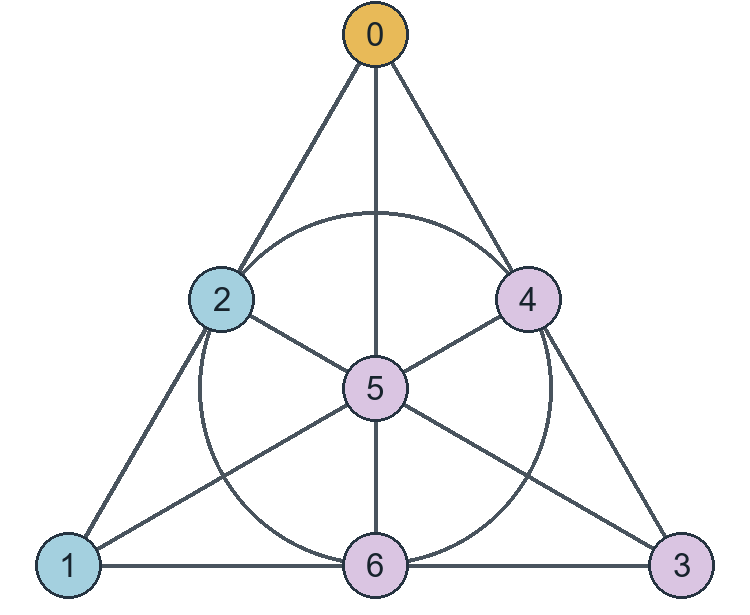
\includegraphics[width=.48\linewidth]{figures/fano.png}}
\caption{Un sistema triple de Steiner de orden siete. Las seis rectas representan los bloques 012, 034, 136, 056, 145 y 235. La circunferencia representa 246. Por cada punto pasan tres bloques.}
\end{figure}

En 1999, Colbourn, Dinitz y Rosa plantearon la Conjetura 2.7: realizar cada perfil admisible de tres clases {[}3{]}. Construyeron los perfiles permitidos de orden menor que 1000. Dinitz y Stinson retomaron el problema sin restricción de orden como su Conjetura 1.4 {[}4{]}. Aquí fijamos los tamaños de clase y contamos qué color se repite en cada bloque. El espectro cromático estudiado por Gionfriddo, Guardo, Milazzo y Voloshin para sistemas pequeños responde a otra pregunta: cuántos colores admite un sistema ya fijado {[}5{]}.

Sea \(t=N_{AAC}\). Cada par interno de \(A\) pertenece a un bloque \(AAB\) o \(AAC\). Cada par entre \(A\) y \(C\) pertenece a un bloque \(AAC\) o \(ACC\), y cada uno de estos bloques aporta dos pares entre clases. De ahí sale la primera fila. Al contar los pares de las otras clases se obtienen, en orden, las dos siguientes. \[\begin{aligned}
N_{AAB}&=\binom a2-t, &N_{ACC}&=ac/2-t,\\
N_{ABB}&=ab/2-N_{AAB}, &N_{BBC}&=\binom b2-N_{ABB},\\
N_{BCC}&=bc/2-N_{BBC}, &N_{ACC}+N_{BCC}&=\binom c2.
\end{aligned}\] La última igualdad permite comprobar la compatibilidad de los conteos. Al sustituir, expresa que hay tantos pares del mismo color como bloques. Con \(n=a+b+c\), equivale a \[a^2+b^2+c^2-ab-ac-bc=n.\] Llamaremos \emph{admisible} a un perfil de entradas positivas que satisfaga esta identidad, con \(n\equiv1,3\pmod6\) y sin dos entradas iguales a 2. Son las condiciones sobre los tamaños de clase estudiadas por Colbourn, Dinitz y Rosa {[}3{]}.

\Needspace{9\baselineskip}\textbf{Teorema 1 (espectro exacto).} Existe un \(n_0\) tal que, para todo perfil admisible \((a,b,c)\) de orden \(n\ge n_0\), un entero \(t\ge0\) es el número de bloques \(AAC\) de algún sistema sobre las clases prescritas si y solo si \[0\le t\le\binom a2,\qquad
L(a,b,c;t),\qquad L\left(a,c,b;\binom a2-t\right).\] La sección 2 define \(L\) por medio de enteros. Intercambiar \(B\) y \(C\) convierte los bloques \(AAB\) en \(AAC\). Por eso comprobamos la misma condición dos veces, una para cada elección del tercer color.

Los seis conteos pueden ser enteros no negativos y, aun así, resultar imposibles. Para \((a,b,c)=(4,6,9)\), el valor \(t=0\) da \((6,0,6,9,18,18)\) en el orden \(AAB,AAC,ABB,BBC,ACC,BCC\). Fijemos un punto de \(A\). Tiene nueve pares con \(C\). Un bloque \(ACC\) que pasa por él cubre dos de esos pares y un bloque \(AAC\) cubre uno. Por paridad, al menos un bloque \(AAC\) debe pasar por cada punto de \(A\). Sumando en \(A\) obtenemos \(2t\ge4\). El ejemplo muestra la obstrucción local en orden 19. La suficiencia que sigue vale uniformemente en el perfil a partir de cierto orden.

\subsection{2. Los pares que pasan por un punto}\label{los-pares-que-pasan-por-un-punto}

Empecemos en un punto de \(A\). Un bloque \(AAB\) que pasa por él aporta un vecino en \(A\) y uno en \(B\). Un bloque \(AAC\) aporta uno en \(A\) y ninguno en \(B\). Un bloque \(ABB\) aporta dos en \(B\) y ninguno en \(A\). Al restar los dos números de vecinos desaparece la contribución de \(AAB\). Haremos esa misma resta en cada clase.

Numeremos las clases en orden cíclico, con \((s_0,s_1,s_2)=(a,b,c)\) e índices módulo 3. Para cada punto \(u\) de la clase \(i\), sea \(m_u\) el número de bloques \(ii(i+2)\) que pasan por \(u\), y sea \(k_u\) el número de bloques \((i+1)(i+1)i\) que tienen a \(u\) como único punto de su clase. Escribamos \(h_u\) para el número de bloques \(ii(i+1)\) que pasan por él. Contemos primero los vecinos de \(u\) en su propia clase y después en la siguiente: \[s_i-1=h_u+m_u,\qquad s_{i+1}=h_u+2k_u.\] La resta elimina \(h_u\). Si \(\alpha_i=s_i-1-s_{i+1}\), queda \(m_u=\alpha_i+2k_u\).

Los bloques que cuenta \(K_i\) tienen clase repetida \(i+1\) y tercer punto en la clase \(i\). Escribamos \(K_i=\sum_{u\in i}k_u=s_iq_i+r_i\), con \(0\le r_i<s_i\), y pongamos \(d_i=\alpha_i+2q_i\). Cada entero \(k_u\) es al menos \(\lceil-\alpha_i/2\rceil\). Su promedio satisface esa cota inferior entera y también la satisface su parte entera \(q_i\). Luego \(d_i\ge0\). Al sumar los \(m_u\) en la clase \(i\), cada par interno que pertenece a un bloque \(ii(i+2)\) se cuenta por sus dos extremos. Hay \(K_{i+2}\) pares de esa clase, uno por bloque. Así obtenemos \[s_id_i+2r_i=2K_{i+2}.\]

Si \(d_i=0\), todos los grados \(m_u=2(k_u-q_i)\) son pares. Los pares internos que acabamos de contar forman un grafo simple con esos grados y exactamente \(r_i\) aristas. Si tiene alguna arista, contiene un ciclo, y un ciclo en un grafo simple requiere al menos tres aristas. Este es el origen de los restos prohibidos 1 y 2.

\textbf{Definición.} Se cumple \(L(a,b,c;t)\) cuando existen enteros no negativos \(d_i,q_i,r_i\) que satisfacen, para cada \(i\), \[\begin{aligned}
 r_i&<s_i, & d_i&=s_i-1-s_{i+1}+2q_i,\\
 s_id_i+2r_i&=2(s_{i+2}q_{i+2}+r_{i+2}),&
 d_i=0&\ \Longrightarrow\ r_i\notin\{1,2\},
\end{aligned}\] y además \(cq_2+r_2=t\). La última ecuación fija el total de bloques cuyo color repetido es \(A\) y cuyo tercer punto está en \(C\). Para evaluar el criterio se parte de \(K_2=t\). Al sustituir la expresión de \(d_i\) se obtiene \(K_{i+2}=K_i+s_i\alpha_i/2\), que determina los otros dos totales. Se divide cada \(K_i\) por \(s_i\) y se comprueban las condiciones anteriores. El conteo en cada punto demuestra la necesidad del criterio, primero en el orden dado y después intercambiando \(B,C\).

\textbf{El cálculo en orden 19.} Volvamos al perfil \((4,6,9)\). Las diferencias \(\alpha_i\) valen \(-3,-4,4\). A partir de \(K_2=t\), la relación de la definición da \(K_1=t+18\) y después \(K_0=t+6\). Si \(t=0\), al dividir \(K_0=6\) por 4 resulta \(q_0=1\). Entonces \(d_0=-3+2=-1\), un grado imposible. El criterio detecta así el mismo impedimento que encontramos al contar los nueve vecinos de cada punto de \(A\). Para \(t=2\), en cambio, la división da \(q_0=2\), \(r_0=0\) y \(d_0=1\). Esa obstrucción concreta desaparece. En orden 19, el cálculo ilustra la condición necesaria; para la prueba de suficiencia usaremos la hipótesis de orden grande.

\subsection{3. Dónde interviene la absorción física tipada}\label{duxf3nde-interviene-la-absorciuxf3n-fuxedsica-tipada}

Representemos cada par por una arista del grafo completo sobre los puntos. Realizar el perfil equivale a descomponer las aristas en triángulos de los seis tipos permitidos. Aplicaremos el Teorema T de Traverso Gianini {[}1{]} tanto al grafo completo como a grafos a los que ya hemos quitado pares. Sus hipótesis deben verificarse en el grafo donde se van a elegir los triángulos.

{\Needspace{23\baselineskip}\begin{longtable}[]{@{}
  >{\raggedright\arraybackslash}p{(\linewidth - 2\tabcolsep) * \real{0.5000}}
  >{\raggedright\arraybackslash}p{(\linewidth - 2\tabcolsep) * \real{0.5000}}@{}}
\toprule\noalign{}
\begin{minipage}[b]{\linewidth}\raggedright
Hipótesis de T
\end{minipage} & \begin{minipage}[b]{\linewidth}\raggedright
Qué hay que comprobar en el grafo
\end{minipage} \\
\midrule\noalign{}
\endhead
\bottomrule\noalign{}
\endlastfoot
H1. Cubrimiento fraccionario & Dar a cada triángulo permitido un peso entre \(1/(Cn)\) y \(C/n\). En cada arista, los pesos de los triángulos que la contienen deben sumar uno. \\
H2. Retículo entero & Escribir el vector de aristas del grafo como combinación entera de los vectores de aristas de triángulos permitidos. Los coeficientes pueden ser negativos. \\
H3. Vecinos comunes & Dados dos puntos distintos y una tercera clase permitida, encontrar en ella al menos \(\alpha n\) vecinos de ambos puntos. \\
H4. Bisagras & Para cada par de triángulos permitidos que comparten una arista, existe un orden \(6\le i\le h\) para el que hay al menos \(\alpha n^{i-4}\) bisagras de exactamente \(i\) vértices. \\
\end{longtable}
}

\textbf{Resultados de absorción {[}1, §§1, 2.3{]}.} Reproducimos los enunciados con la numeración de ecuaciones original. Aquí \(M_\mu(w)\) suma los pesos de la semilla contra \(w\), y \(P_\mu\) suma los productos de cuatro pesos sobre las configuraciones de Pasch. Las declaraciones son main\_theorem\_T y main\_theorem\_T\_with\_triangle\_monitors\_and\_pasch.

\textbf{Teorema T.} Fijemos \(I,\mathcal F,\alpha,C,h\) con \(\alpha>0\), \(C\geq1\) y \(h\geq6\). Existe un entero \(n_0\) tal que todo grafo etiquetado G de orden \(n\geq n_0\) que satisface H1--H4 admite una descomposición en triángulos permitidos.

\textbf{Teorema T+.} Fijemos \(I,\mathcal F,\alpha,C,h\) como en el Teorema T, junto con \(\eta>0\) y un entero \(q\geq0\). Existe un entero \(n_0\) tal que lo siguiente se cumple para todo grafo etiquetado G de orden \(n\geq n_0\) y toda semilla especificada \(\mu\) que satisface H1, siempre que se cumplan H2--H4. Para toda familia finita \((w_j)_{j\in\mathcal J}\) con

\[|\mathcal J|\leq n^q,
\qquad |w_j(Q)|\leq1\quad(j\in\mathcal J,\ Q\in\mathcal T),          \tag{2.9}\]

existe una descomposición en triángulos permitidos \(\mathcal D\) tal que

\[\left|\sum_{Q\in\mathcal D}w_j(Q)-M_\mu(w_j)\right|
\leq\eta n^2\qquad(j\in\mathcal J),                                \tag{2.10}\]

y

\[|P(\mathcal D)-P_\mu|\leq\eta n^2.                                \tag{2.11}\]

Esta prueba del espectro da un umbral existencial. Las cotas numéricas de los lemas siguientes no proporcionan el valor del umbral de T ni el de T+ con Pasch.

\subsubsection{3.1. Cómo elegir los pesos}\label{cuxf3mo-elegir-los-pesos}

Sea \(w_{AAC}\) el peso de cada triángulo de ese tipo. Para un par interno de \(C\) hay \(a\) terceros puntos en \(A\) y \(b\) en \(B\). Repartamos la carga por mitades entre ambas clases: ponemos \(w_{ACC}=1/(2a)\) y \(w_{BCC}=1/(2b)\). Fijemos ahora un par \(AC\). El tercer punto puede ser uno de los otros \(a-1\) puntos de \(A\) o uno de los otros \(c-1\) puntos de \(C\). Al resolver la ecuación de carga de ese par, y después la de un par \(BC\), resulta \[w_{AAC}=\frac{1-(c-1)/(2a)}{a-1},\qquad
w_{BBC}=\frac{1-(c-1)/(2b)}{b-1}.\] Los pares internos de \(A\) y de \(B\) fijan los últimos dos pesos: \[b w_{AAB}=1-cw_{AAC},\qquad a w_{ABB}=1-cw_{BBC}.\] Falta comprobar la carga de los pares \(AB\). En cada triángulo hay dos pares entre clases y uno interno. Por la identidad del perfil, el grafo completo también tiene el doble de pares entre clases que internos. Todos los pares salvo los \(AB\) ya tienen carga uno, y los \(AB\) tienen la misma carga entre sí. Por tanto, también en ellos la carga es uno. El lema de los pesos acota estas seis expresiones entre \(1/(4n)\) y \(4/n\) para \(n\ge400\). Para ello usa que \((a-b)^2+(b-c)^2+(c-a)^2=2n\): cada tamaño de clase difiere de \(n/3\) en a lo sumo \(O(\sqrt n)\).

\subsubsection{3.2. La condición entera y los intercambios locales}\label{la-condiciuxf3n-entera-y-los-intercambios-locales}

Veamos dos de estas comprobaciones sobre los vectores de aristas. Para H2 tomamos el cociente del grupo abeliano libre sobre las aristas por el subgrupo generado por los vectores de los triángulos permitidos. En el cociente, cada terna permitida da \([xy]+[xz]+[yz]=0\). Cada clase tiene al menos tres puntos. Por ejemplo, fijemos dos puntos \(w,w'\) fuera de una clase y escribamos \(D_x=[xw]-[xw']\) para los puntos \(x\) de esa clase. Restemos las relaciones de los triángulos \(xyw\) y \(xyw'\). Resulta \(D_x+D_y=0\) para cualesquiera \(x,y\) distintos en la clase. Al usar un tercer punto se obtiene \(D_x=D_y\) y \(2D_x=0\). De aquí vienen los términos de orden a lo sumo dos que aparecerán al sumar las aristas. Fijemos representantes \(o_i\) de las tres clases. Para \(u\) de color \(i\) pongamos \(e_u=[uw]-[o_iw]\), con \(w\) fuera de la clase \(i\). La identidad anterior para \(D_x\) muestra que la diferencia no depende de \(w\): al restar sus valores en \(w,w'\) se obtiene \(D_u-D_{o_i}=0\). Elijamos dos puntos distintos \(w,w'\) de una misma clase externa. Al restar las relaciones de los triángulos \(uww'\) y \(o_iww'\) resulta \(e_u+e_u=0\). En una arista entre clases sustituimos cada extremo por su representante y obtenemos \([uv]=[o_io_j]+e_u+e_v\). Para una arista interna usamos \([uv]=-[uw]-[vw]\) y \(2e_w=0\). El término constante es \(-2[o_io_j]\), independiente de la otra clase \(j\). Los tres dobles de las constantes entre clases coinciden; llamemos \(\gamma\) a su valor. Al sumar sobre todos los pares, cada \(e_u\) aparece \(n-1\) veces y se anula. El coeficiente restante de \(\gamma\) es \[\tfrac12(ab+bc+ca)-\binom a2-\binom b2-\binom c2.\] Como \(n\) es impar, hay una o tres clases impares, y la identidad cuadrática excluye tres. Cada producto entre clases es par y el coeficiente se anula por la identidad del perfil. Así se obtiene la pertenencia al retículo físico antes de construir ningún sistema.

Para H4, sean \(uva,uvb\) dos triángulos permitidos sobre cuatro puntos distintos (aquí \(a,b\) designan vértices). Tomemos otros dos puntos \(x,y\) en las clases de \(u,v\), respectivamente. Pongamos \(J=\{uy,xv,xy,xa,xb,ya,yb\}\). Al añadir \(ua,va\) a \(J\), las nueve aristas se reparten en \(uya,xva,xyb\). Si añadimos \(ub,vb\), se reparten en \(uyb,xvb,xya\). Cada triángulo tiene uno de los dos tipos iniciales. Las elecciones distintas dan al menos \(n^2/32\) bisagras en el grafo completo. En el grafo residual se repite la construcción excluyendo los puntos que hayan perdido alguna adyacencia necesaria.

\textbf{Proposición 3.2 (el grafo completo).} Todo perfil admisible de orden suficientemente grande tiene una realización. \emph{Demostración.} Para H3 sirven todos los puntos de la clase prescrita salvo los dos puntos fijados. Si \(n\ge400\), cada clase tiene al menos \(n/4+2\) puntos. Esta observación y el conteo anterior de bisagras dan H3 y H4 con \(\alpha=1/32\) y bisagras de orden 6. Tomemos el mayor entre 400 y el umbral de T {[}1{]} para estos parámetros y \(C=4\). Las secciones 3.1 y 3.2 verifican las cuatro hipótesis. T divide las aristas en triángulos permitidos. Al tomar esos triángulos como bloques obtenemos exactamente un bloque por par, con las clases originales.

En H3 los dos puntos distintos pueden no ser adyacentes: se exige la cota cuando sus dos etiquetas y la tercera propuesta forman un multiconjunto permitido.

\subsubsection{3.3. Qué cambia cuando reservamos algunos pares}\label{quuxe9-cambia-cuando-reservamos-algunos-pares}

Para determinar el espectro exacto hay que reservar algunos pares antes de aplicar la absorción. El teorema de descomposición por partes de Keevash {[}6, Teorema 5.15{]} da un criterio general de existencia en orden grande. Aquí necesitamos además controlar cuántos triángulos de cierto tipo añade la completación. T+ {[}1{]} estima ese número a partir de los pesos: para el indicador de \(AAC\), la diferencia entre el conteo y la suma ponderada es a lo sumo \(\eta n^2\).

Al eliminar pares hay que comprobar H1 de nuevo. Sea \(\mathsf A\) el operador que transforma los pesos de los triángulos en las cargas de las aristas. Si una primera elección de pesos da cargas \(\mathsf A\mu\), la corrección ha de resolver \(\mathsf A z=\mathbf1-\mathsf A\mu\) en las aristas restantes. En el vector de un triángulo hay dos pares entre clases por cada par interno. Por tanto, toda carga de la imagen satisface \(\sum_{\rm entre} f=2\sum_{\rm internos} f\). La carga buscada satisface la misma igualdad por la admisibilidad y porque se han restado vectores de triángulos reservados. La diferencia pertenece así al subespacio en que está definido el inverso. Para los seis tipos, el lema del inverso acotado en el grafo completo limita la corrección por una constante multiplicada por el error máximo de carga y dividida por \(n\). Tras un borrado disperso se restringe una corrección a los triángulos que quedan y se corrige el nuevo error, menor que el anterior. La convergencia geométrica da una semilla exacta y la cota sobre la corrección total conserva la positividad. El uso de un inverso y una estimación de perturbación tiene precedentes en descomposiciones fraccionarias {[}7,8{]}. Si se restringen los tipos, hay que identificar el subespacio de cargas en que la ecuación tiene solución. Esa distinción será importante cerca de los extremos.

\textbf{Lema 3.3 (inversa para seis tipos; bri\_of\_balanced).} Si los tres tamaños son al menos \(m\ge512\) y \(n\le4m\), toda carga real \(f\) sobre los pares cuya suma entre clases duplica la suma interna admite una elección lineal de pesos \(z\) en los triángulos permitidos, con \(\mathsf A z=f\) y \(\|z\|_\infty\le52000\|f\|_\infty/n\). El apéndice A desarrolla la construcción y las dos cotas de norma.

Para ver de dónde sale 52000, llamemos \(W\) al subespacio de las cargas equilibradas. El operador aproximado \(\Phi_0\) asigna pesos a los triángulos con \(\|\Phi_0 f\|_\infty\le26000\|f\|_\infty/n\) en \(W\). Al sumar esos pesos sobre cada arista, el error es a lo sumo \(\|f\|_\infty/2\). Por tanto, \(F=\mathsf A\Phi_0\) lleva \(W\) en sí mismo y \(\|Ff\|_\infty\ge\|f\|_\infty/2\). En dimensión finita esto hace que \(F\) sea invertible en \(W\). El operador exacto \(\Phi_0 F^{-1}\) tiene entonces una cota a lo sumo dos veces mayor. Las estimaciones para \(\Phi_0\) se demuestran en norm\_err\_le (BRIAssembly) y abs\_Phi0\_le (BRIFinal), en la carpeta CDRBicolour/Absorption del archivo de fuentes común.

\subsection{4. Cómo corregir el error de uno en uno}\label{cuxf3mo-corregir-el-error-de-uno-en-uno}

Supongamos que cada uno de los seis conteos requeridos es al menos \(\delta n^2\), con \(\delta>0\) fijo. Etiquetemos nueve puntos: \(0,1,2\) en \(A\), \(3,4,5\) en \(B\) y \(6,7,8\) en \(C\). Cada cadena de la tabla representa una terna. Las dos filas descomponen los mismos pares.

{\begin{longtable}[]{@{}llr@{}}
\toprule\noalign{}
Elección & Ternas, agrupadas por su primer punto & \(AAC\) \\
\midrule\noalign{}
\endhead
\bottomrule\noalign{}
\endlastfoot
Baja & 015, 023, 067; 127, 134, 168; 356, 378, 458 & 1 \\
Alta & 016, 027, 035; 123, 145, 178; 348, 367, 568 & 2 \\
\end{longtable}
}

Por ejemplo, la terna 015 de la primera fila usa los pares 01, 05 y 15, que en la segunda aparecen en 016, 035 y 145. Desglosando las otras ocho ternas de igual manera se obtienen los mismos 27 pares distintos en ambas filas. En la fila baja solo 127 es de tipo \(AAC\); en la alta lo son 016 y 027. El intercambio entre filas conserva las aristas cubiertas y modifica \(t\) en una unidad.

\begin{figure}[htbp]
\centering
\pandocbounded{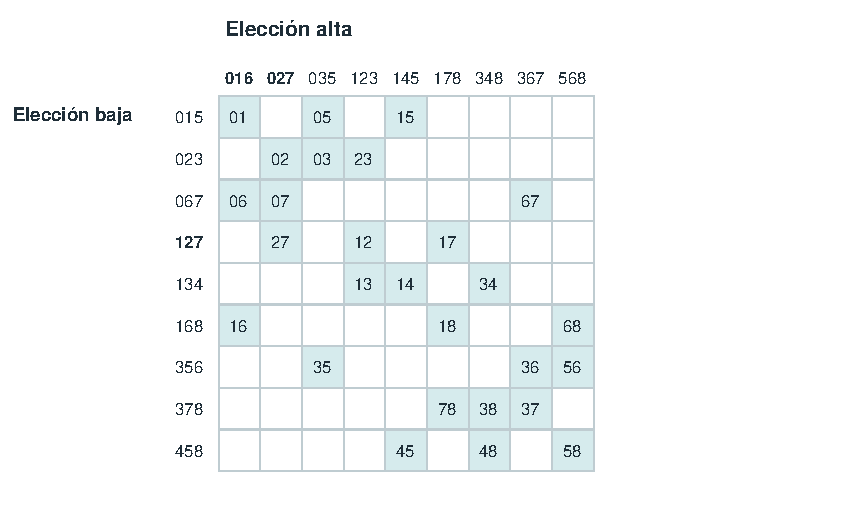
\includegraphics[width=.89\linewidth]{figures/trade_es.pdf}}
\caption{Los mismos 27 pares en dos descomposiciones. Cada casilla ocupada indica el par común a la terna de su fila y la de su columna. Las ternas en negrita son de tipo AAC.}
\end{figure}

\textbf{Lema 4.1 (copy\_edge, degL\_leave).} Para cada primo \(m>8\) con \(\min(a,b,c)\ge3m\), se pueden reservar \(m^2\) copias del intercambio sin aristas en común. Ambas elecciones cubren las mismas aristas en cada copia. El grado máximo de la unión es a lo sumo \(81m\), una cota holgada. Como \(m\) es impar, el objetivo \(m_0=t-3m^2/2\) es semientero; solo el número de elecciones altas debe ser entero.

El primo y la tolerancia se pueden elegir en el orden necesario. Escribimos \(K=52000\), \(C_0=64+2/\delta\), y fijamos \(\lambda=1/(10^9 C_0^2)\) y \(\eta=\lambda^2/16\) antes de tomar el umbral de T+. Para \(n\) grande sea \(r=\lfloor\lambda n\rfloor\). Por el postulado de Bertrand hay un primo \(r<m\le2r\); por tanto \(m\) es suficientemente grande para la construcción, \(3m\le\min(a,b,c)\) y \(\eta n^2\le m^2/4\). Cada conteo por tipo es afín en \(t\) con pendiente \(1\) o \(-1\): mover \(t\) en a lo sumo \(\delta n^2/2\) conserva al menos la mitad del margen inicial de cada tipo. Los desplazamientos que siguen son a lo sumo \(3m^2/2+2(4K+1)C_0\,81mn\). Al sustituir \(m\le2\lambda n\), \(K=52000\), \(C_0\ge64\) y \(1/C_0\le\delta/2\) quedan dentro de ese margen.

Necesitaremos toda una familia de semillas en el grafo completo. Sustituimos \(t\) por un número real \(\tau\) en los seis conteos de pares de la sección 1 y llamamos \(N_X\) a las masas que resultan. Para un tipo \(X=iij\) hay \(T_X=\binom{s_i}{2}s_j\) ternas disponibles, donde \(s_i,s_j\) son los tamaños de las clases. Asignamos peso \(N_X/T_X\) a cada terna de ese tipo. La masa en \(AAC\) es exactamente \(\tau\). Las seis ecuaciones de la sección 1 dan como carga total de cada clase de pares el número de pares de esa clase. Las permutaciones dentro de cada clase de vértices conservan los pesos y llevan cualquier par a cualquier otro de su misma clase. Por eso cada par tiene carga uno. Para las dos elecciones de \(\tau\) que siguen, el margen disponible deja \(N_X\ge(\delta/2)n^2\). Además, el conteo de pares internos da \(N_X\le n^2/2\), y \(n^3/128\le T_X\le n^3\) porque cada clase tiene al menos \(n/4+2\) puntos. Al dividir obtenemos pesos entre \(1/(C_0 n)\) y \(C_0/n\) con \(C_0=64+2/\delta\). Esta es la familia construida en SeedCounts.

El lema de colocación del intercambio da \(M=m^2\) copias sin aristas en común, con \(m\) primo de orden \(\lambda n\) y \(\lambda\) suficientemente pequeño en función de \(\delta\). Para ver por qué dos copias no pueden compartir un par, demos a cada una de las nueve posiciones un grupo distinto de \(m\) puntos. La copia \((s,z)\) usa el punto \(s+iz\) del grupo \(i\), con aritmética módulo \(m>8\). Coincidir en dos grupos \(i\ne j\) da \((i-j)(z-z')=0\), luego \(z=z'\) y después \(s=s'\). Quitemos las aristas reservadas, que son las mismas para cualquiera de las elecciones. Si elegimos siempre la fila baja, las copias aportan \(M\) bloques del tipo contado; si elegimos siempre la alta, aportan \(2M\). Por eso apuntamos, en el grafo restante, al valor intermedio \(m_0=t-3M/2\). Veamos cómo obtener esa masa después de retirar las aristas reservadas. Escribamos \(\Delta=81m\) para la cota del grado eliminado, \(K=52000\) para la constante del inverso de los seis tipos y \(C_0=64+2/\delta\). Si la semilla inicial tiene masa \(\tau\), el lema de corrección da en el grafo restante una masa \(b_\tau\) que cumple \[|b_\tau-\tau|\le E,\qquad E=(4K+1)C_0\Delta n.\] La masa de la semilla perdida al borrar triángulos es a lo sumo \(C_0\Delta n/2\). En cada arista superviviente se pierden a lo sumo \(2\Delta\) terceros puntos posibles, por lo que el déficit de carga es a lo sumo \(2\Delta C_0/n\). La cota del inverso y el factor dos de la serie geométrica del apéndice A dan una masa total de corrección a lo sumo \(4KC_0\Delta n\). La suma queda acotada por \((4K+1)C_0\Delta n\), como se afirmó. El lema de colocación elige \(\lambda=1/(10^9 C_0^2)\) antes de fijar \(n\); así queda margen suficiente dentro de \(\delta n^2\) para usar tanto \(\tau_-=m_0-2E\) como \(\tau_+=m_0+2E\). Aplicando la estimación a cada semilla obtenemos \[b_{\tau_-}\le m_0-E,\qquad b_{\tau_+}\ge m_0+E.\] Pongamos \(s=(m_0-b_{\tau_-})/(b_{\tau_+}-b_{\tau_-})\). Se tiene \(0\le s\le1\). Combinamos las dos semillas corregidas con coeficientes \(1-s,s\). En cada arista restante la carga es \((1-s)+s=1\). Los pesos siguen dentro de sus cotas y la masa de los triángulos \(AAC\) es ahora exactamente \(m_0\).

Apliquemos T+ al indicador del tipo \(AAC\). Elegimos la tolerancia de modo que el conteo residual \(D\) satisfaga \(|D-m_0|\le M/4\). Tomemos la fila alta en exactamente \(k=t-M-D\) copias. Este número es entero y cumple \[k=M/2+(m_0-D)\in[M/4,3M/4].\] Disponemos de suficientes copias para ambas elecciones. En el sistema completo el conteo vale \(D+(M-k)+2k=t\). Así se pasa de la aproximación de Paper III a la igualdad buscada.

\subsection{5. Qué hacer cuando escasean tres tipos}\label{quuxe9-hacer-cuando-escasean-tres-tipos}

\textbf{Lema 5.1 (exists\_graph).} Si \(4d+64\le s\), \(0\le r<s\), la imparidad de \(d\) exige que \(s\) sea par, y \(d=0\) exige \(r\notin\{1,2\}\), existe un grafo simple sobre las posiciones cíclicas \(0,\ldots,s-1\) con grado \(d+2\) en las primeras \(r\) posiciones consecutivas y \(d\) en las restantes.

\textbf{Lema 5.2 (lower\_packing).} Dado un perfil admisible con testigos de \(L\), supongamos \(4d_i+64\le s_i\) y \(d_i+3\le s_{i+2}\) en cada clase. Existe un empaquetamiento de tipos minoritarios con exactamente \(cq_2+r_2\) bloques \(AAC\). En cada punto de clase \(i\), para algún \(e\in\{0,1\}\), los grados cubiertos hacia \(i,i+1,i+2\) son \(d_i+2e,2(q_i+e),d_i+2e\), respectivamente. La paridad de \(s_i d_i=2K_{i+2}-2r_i\) da la condición del lema 5.1.

\textbf{Lema 5.3 (physical\_maj).} Supongamos que cada clase está presente y que cada cuatro puntos, admitiendo repeticiones, tienen en el residuo un vecino común en cada clase prescrita. Si en cada punto coinciden los grados interno y hacia la clase siguiente, y es par el grado hacia la clase anterior, el vector de aristas residuales pertenece al retículo entero generado por los triángulos mayoritarios restantes.

\textbf{Lema 5.4 (corner\_residual\_seed).} En un perfil admisible con \(n\ge10^{24}\), retiremos un conjunto de pares de grado máximo \(\Delta\) con \(10^{13}\Delta\le n\). Si en cada punto coinciden los grados restantes interno y hacia la clase siguiente, los triángulos mayoritarios admiten una semilla exacta difusa de constante 8.

Cerca del extremo inferior puede faltar margen para dar peso a los seis tipos. Colocaremos primero \emph{todos} los bloques de los tipos \(ii(i+2)\). El lema de colocación parte de las relaciones enteras de \(L\) y de la cota \(10^{15}(d_i+q_i+1)\le n\) en cada clase. Dentro de la clase \(i\) se construye un grafo simple con \(r_i\) vértices de grado \(d_i+2\) y los demás de grado \(d_i\). La suma de grados es \(s_id_i+2r_i=2K_{i+2}\), exactamente el número de extremos que se necesitan. Cuando el grado base es cero, los dos restos excluidos en la sección 2 corresponden precisamente a la obstrucción de una o dos aristas. Usamos el teorema de coloración de aristas de Vizing y el reequilibrio equitativo {[}9,10{]}. Una coloración propia y equitativa de las aristas asigna a cada par interno un tercer punto de la clase \(i+2\). Al ser propia, evita repetir un par entre clases. Cada clase de aristas contiene \(q_{i+2}\) o \(q_{i+2}+1\) aristas. Reetiquetando se hacen coincidir las cargas mayores con los vértices designados de mayor grado en esa clase. Los tres grafos dan así un empaquetamiento con los conteos minoritarios prescritos y sin aristas repetidas.

\textbf{Cómo se construye el grafo interno.} Coloquemos los \(s_i\) vértices en un círculo. Para cada salto elegido \(0<j<s_i/2\), unimos cada vértice con los situados a distancia \(j\) a derecha e izquierda. Con cada salto, todos los grados aumentan en dos. Si el orden es par, un emparejamiento de puntos diametralmente opuestos permite añadir uno más. Para aumentar en dos el grado de \(r_i\ge3\) vértices, trazamos un ciclo sobre ellos: recorremos las posiciones pares en orden creciente y regresamos por las impares en orden decreciente. El ciclo solo usa saltos de longitud uno o dos, que se dejan libres al elegir los saltos iniciales. Con uno o dos vértices elegidos no hay ciclo. El lema usa entonces una arista \(xy\) y la sustituye por \(xu,uy\), ambas libres. Los grados de \(x,y\) se conservan y el de \(u\) aumenta en dos. Esta operación necesita una arista inicial; de ahí la excepción cuando \(d_i=0\). Bajo la hipótesis de dispersión, el lema permite hacer estas elecciones sin repetir aristas. Después, la coloración propia asigna a cada arista su tercer punto.

Consideremos un vértice \(u\) de la clase \(i\) que figura \(k_u\) veces como tercer punto y tiene grado interno \(m_u=\alpha_i+2k_u\). Después de colocar los bloques le quedan \(s_i-1-m_u\) vecinos en su clase y \(s_{i+1}-2k_u\) en la siguiente. Esas cantidades son iguales. Su grado total restante es par: el grado inicial era \(n-1\) y cada triángulo colocado que pasa por \(u\) quita dos aristas. Restar las dos cantidades iguales de vecinos deja un grado par hacia la clase anterior, como exige cubrir esas aristas de dos en dos cuando \(u\) aporta el tercer punto. En el grafo residual denso, el lema del retículo de los tipos mayoritarios deduce H2 precisamente de ese equilibrio y esa paridad.

El cálculo en el retículo explica por qué bastan esas dos condiciones. En el cociente por los triángulos mayoritarios, el lema del retículo escribe la clase de una arista interna \(uv\) como \(-\phi(u)-\phi(v)\), y la de una arista \(uv\) de \(i\) a \(i+1\) como \(\phi(u)+\psi(v)\), con \(2\psi(v)=0\). Al sumar sobre las aristas, el coeficiente de \(\phi\) en cada vértice es el grado hacia la clase siguiente menos el grado interno: vale cero. El coeficiente de \(\psi\) es el grado hacia la clase anterior: es par. La suma de todas las clases de aristas se anula en el cociente. Eso es H2.

Para H1 se comienza con peso \(1/s_{i+1}\) en cada triángulo mayoritario \(ii(i+1)\). En el grafo completo una arista interna recibe carga uno, pues hay \(s_{i+1}\) posibles terceros puntos. Una arista de \(i\) a \(i+1\) recibe carga \((s_i-1)/s_{i+1}\), por las \(s_i-1\) posibles elecciones en \(i\). El error es \(O(n^{-1/2})\). Tras colocar los bloques usamos el inverso de los \emph{tres} tipos mayoritarios en el subespacio de cargas en que coinciden el grado interno y el grado hacia la clase siguiente en cada vértice. El lema de la semilla residual da pesos exactos con constante 8 si el grado eliminado es a lo sumo \(n/10^{13}\) y \(n\ge10^{24}\). Las cotas de la colocación garantizan ese grado. Cada clase prescrita sigue ofreciendo un número lineal de elecciones después de excluir las raíces y los vecinos perdidos, tanto para H3 como para los dos vértices libres de H4. T descompone ahora el grafo restante usando solo los tipos mayoritarios. Todos los bloques \(AAC\) del sistema son, por tanto, los \(t\) que ya colocamos.

\subsubsection{5.1. Por qué estos casos cubren todos los valores admisibles}\label{por-quuxe9-estos-casos-cubren-todos-los-valores-admisibles}

Si se cumple la cota de colocación, el argumento anterior resuelve el extremo inferior. Hagamos ahora la misma prueba intercambiando \(B\) y \(C\). En ese orden obtenemos \(\binom a2-t\) bloques con el otro color en el tercer punto, de modo que en el orden original quedan exactamente \(t\). Falta ver qué ocurre si la cota falla en ambos órdenes. Demostraremos que entonces los seis tipos abundan lo suficiente para aplicar la sección 4.

\textbf{Lema 5.5 (large\_counts\_R, aplicado a perfiles).} Para todo perfil admisible de orden \(n\ge10^{40}\) que cumpla \(L\), si \(10^{15}(d_j+q_j+1)>n\) para algún \(j\), los tres conteos asociados satisfacen \(K_i\ge n^2/10^{17}\). \emph{Demostración.} Tomemos \(n\ge10^{40}\) en esta estimación. Como \((s_i-s_{i+1})^2\le2n\), se cumple \(|\alpha_i|\le\sqrt{2n}+1\le n/10^{17}\). Que la cota falle en una clase \(j\) significa que \(n<10^{15}(d_j+q_j+1)\). Sustituyamos \(d_j=\alpha_j+2q_j\). La estimación anterior y la desigualdad \(1\le n/10^{17}\) dan \(3q_j>n/10^{15}-2n/10^{17}\), y por tanto \(q_j\ge n/(6\cdot10^{15})\). Como \(s_j\ge n/4\), se obtiene \(K_j\ge n^2/(24\cdot10^{15})\).

Usemos ahora \(K_{i+2}-K_i=s_i\alpha_i/2\). En un paso se pierde a lo sumo \(n^2/(2\cdot10^{17})\). Bastan dos pasos para alcanzar cualquiera de las otras clases. Por consiguiente, cada uno de los tres conteos satisface \[K_i\ge\frac{n^2}{24\cdot10^{15}}-\frac{n^2}{10^{17}}\ge\frac{n^2}{10^{17}}.\] Al intercambiar las clases se obtiene la misma cota para los otros tres tipos. Podemos, pues, aplicar la sección 4 con \(\delta=10^{-17}\). Basta elegir el orden por encima de todos los umbrales usados en las construcciones. Esto prueba la suficiencia y, junto con la necesidad demostrada en la sección 2, termina la prueba del teorema 1.

\subsection{6. Otras prescripciones}\label{otras-prescripciones}

\textbf{Teorema 6.1 (cdr\_completion).} Lindner y Rosa estudiaron los posibles \emph{tamaños} del conjunto de bloques comunes de dos sistemas {[}11{]}. Aquí fijamos la partición y prescribimos los bloques comunes uno a uno. Sea \(P\) un empaquetamiento de triángulos permitidos sin aristas comunes. Llamemos \(\Delta\) al grado máximo del grafo de pares ya cubiertos. Para perfiles admisibles grandes, \(6656000\Delta\le n\) basta para completar \(P\). La estimación de la semilla residual da H1 y retirar los triángulos de \(P\) equivale a restar generadores enteros en H2. Los conteos de vecinos y bisagras resisten este borrado. Reunir \(P\) y la descomposición residual cubre cada par una vez.

\textbf{Teorema 6.2 (cdr\_prescribed\_intersection).} Para las mismas clases prescritas, un refinamiento da constantes \(K,n_0\) tales que \(n\ge n_0\) y \(K\Delta\le n\) bastan para obtener dos completaciones con intersección \emph{exactamente} igual a \(P\). Se subdividen las clases de color y se completa dos veces lo que queda, con conjuntos disjuntos de tipos refinados. Un bloque común fuera de \(P\) tendría que pertenecer a ambos conjuntos. La prueba completa de este refinamiento es formal; el apéndice B identifica su declaración y sus dependencias.

\textbf{Teorema 6.3 (cdr\_many\_pasch\_counts).} Una configuración de Pasch consta de cuatro bloques sobre seis puntos, cada uno presente dos veces. Para cada \(k\) fijo y todo perfil admisible suficientemente grande hay \(k\) realizaciones con números de Pasch distintos dos a dos. Al perturbar de forma equilibrada una semilla, el conteo ponderado de Pasch es \(A_0+A_2z^2+A_4z^4\), con \(A_4\ge n^2/40^6\). Como función de \(z^2\) es cuadrático. En una malla de \(2k+1\) puntos convenientemente espaciados se obtienen \(k\) valores separados por un múltiplo positivo de \(n^2\) que depende de \(k\). Basta elegir en T+ una tolerancia para Pasch menor que la mitad de esa separación. Los conteos de las realizaciones quedan entonces en intervalos disjuntos. Incluso olvidando los colores, los sistemas son no isomorfos dos a dos.

Como punto de comparación, las construcciones de cintura grande dan sistemas sin ninguna configuración de Pasch {[}12{]}. Aquí mantenemos fijas las tres clases de color y separamos los conteos de varias realizaciones.

\textbf{Teorema 6.4 (realCount\_log\_asymptotic).} Sobre puntos etiquetados con partición fija, sea \(R(a,b,c)\) el número de familias de bloques distintas. Uniformemente para perfiles admisibles grandes se tiene \[\log R(a,b,c)=(1/6+o(1))n^2\log n.\] La construcción de Wilson {[}13{]}, la cota superior por entropía de Linial y Luria {[}14{]} y la enumeración de Keevash {[}15{]} conciernen a sistemas sin restricción de colores. En el conteo presente cada realización ha de respetar la partición fijada. Para la cota superior se eligen \(n(n-1)/6\) bloques entre a lo sumo \(\binom n3\) candidatos y se aplica \(\binom{v}{b}\le(ev/b)^b\). La cota formal aplica Linial--Luria {[}14{]} antes de restringir los colores. Para la cota inferior, wilson\_core usa grupos equilibrados en las tres clases y un STS sobre sus índices. Para cada terna de grupos se eligen cuadrados latinos en celdas seleccionadas por el patrón permitido de colores. Por ello cada terna elegida repite un color. Se prepara un residuo reservado con su propia semilla, vecinos comunes y bisagras, y T lo completa. Las elecciones independientes de cuadrados latinos se recuperan al restringir a las celdas transversales.

\subsection{Apéndice A. Cómo se transfieren las cargas entre aristas}\label{apuxe9ndice-a.-cuxf3mo-se-transfieren-las-cargas-entre-aristas}

\textbf{La inversa para seis tipos (lema 3.3).} Denotamos por \([uv]\) el indicador de una arista y por \([uvw]\) el de un triángulo. Sea \(f\) una carga equilibrada. Por linealidad basta considerar \(\|f\|_\infty=1\); para la carga cero tomamos pesos nulos.

\begin{enumerate}
\def\labelenumi{\arabic{enumi}.}
\tightlist
\item
  Fijada la arista \(uv\), promediamos sobre los siguientes pares ordenados \(w,z\). Si \(u,v\) pertenecen a la clase \(i\), elegimos dos puntos distintos de \(i+1\). En otro caso elegimos \(w\) en la clase de \(u\) y \(z\) en la de \(v\), excluyendo los dos extremos. Llamemos \(P_{uv}\) al conjunto de elecciones y pongamos \(P=(m-1)^2\); entonces \(|P_{uv}|\ge P\). Los cuatro triángulos de \([uvw]+[uvz]-[uwz]-[vwz]\) están permitidos. Su incidencia es \(2[uv]-2[wz]\), pues las otras cuatro aristas aparecen una vez con cada signo. Dividimos por \(2|P_{uv}|\), sumamos sobre \(w,z\), multiplicamos por \(f(uv)\) y sumamos sobre las aristas de entrada. Los pesos \(\Phi_1 f\) así obtenidos reproducen \(f\) menos la carga redistribuida. Fijado un triángulo de salida, cada uno de los cuatro indicadores fija tres de los cuatro vértices de a lo sumo \(3^3\) maneras. Para el vértice libre quedan a lo sumo \(n\) elecciones. Por tanto \(\|\Phi_1 f\|_\infty\le54n/P\).
\item
  Separamos la carga redistribuida en un valor \(G_{ij}\) por tipo de arista y un error local. Para obtener ese valor contamos las mismas clases de destino con el mismo denominador, pero permitimos que la arista de destino toque la de partida. Cada arista aporta a lo sumo \(2/P\). Para una arista de destino fija, solo las que comparten un extremo con ella pueden causar error. Hay a lo sumo \(2n\), lo que da la cota holgada \(8n/P\). Sea \(\ell\) la suma en las aristas entre clases menos el doble de la suma interna. Antes de admitir coincidencias de extremos, la carga redistribuida satisface \(\ell=0\) porque cada transferencia conserva el carácter interno o entre clases de la arista. Para cada entrada se añaden a lo sumo \(2n\) destinos ordenados en la suma de equilibrio: en una arista entre clases el coeficiente es uno, y en una arista interna los destinos se encuentran en la clase siguiente, sin extremos que excluir. Así, \(|\ell(G)|\le 2n^3/P\). Restamos \(\lambda=\ell(G)/(ab+bc+ca)\) de los tres valores entre clases. La carga resultante \(G'\) está equilibrada y \(|\lambda|\le2n^3/(3m^2P)\). Como \(m\ge512\), \(n\le4m\) y \(P\ge m^2/2\), tanto el error local como \(|\lambda|\) son a lo sumo \(1/4\). Además \(|G'_{ij}|\le2n^2/P+1/4\le65\).
\item
  Resolvemos las seis ecuaciones por tipo para la carga corregida. Tomamos \(w_{AAC}=0\); las ecuaciones para \(AA\) y \(AC\) dan \(w_{AAB}=G'_{AA}/b\) y \(w_{ACC}=G'_{AC}/(c-1)\). Las de \(AB\), \(CC\) y \(BB\) dan, por ese orden, \[w_{ABB}=\frac{G'_{AB}-(a-1)w_{AAB}}{b-1},\quad
   w_{BCC}=\frac{G'_{CC}-a w_{ACC}}b,\quad
   w_{BBC}=\frac{G'_{BB}-a w_{ABB}}c .\] La ecuación restante, para \(BC\), se deduce al aplicar \(\ell\) al error: los demás tipos ya tienen la carga exacta y \(bc>0\). Cada denominador es al menos \(m-1\) y toda clase tiene a lo sumo \(6(m-1)\) puntos. A partir de \(B=65\) las sustituciones dan sucesivamente \(B/(m-1)\), \(7B/(m-1)\) y \(43B/(m-1)\). Sumamos estos pesos uniformes a \(\Phi_1 f\) para obtener \(\Phi_0 f\). Como \(m-1\ge n/8\), su norma es a lo sumo \((3456+22360)/n<26000/n\). El paso 2 da \(\|f-\mathsf A\Phi_0 f\|_\infty\le1/2\). El argumento en dimensión finita de la sección 3.3 da ahora \(52000/n\).
\end{enumerate}

\textbf{Potenciales en el grafo residual (lema 5.3).} Trabajamos módulo las sumas enteras de triángulos mayoritarios que sobreviven. Sean \(v,v'\) de la clase siguiente a la de \(u\). Ponemos \(D(u)=[uv]-[uv']\) cuando existen ambas aristas. Si \(uu'\) es arista y ambos extremos son vecinos de \(v,v'\), restar las relaciones de los dos triángulos da \(D(u)+D(u')=0\). Elegimos en la clase de \(u\) otros dos vértices adyacentes entre sí, a \(u\) y a los dos vértices de la clase siguiente. Bastan dos elecciones de vecino común, la segunda con cuatro vértices fijados. Aplicando la relación en los tres lados resulta \(2D(u)=0\). Si dos extremos iniciales no son adyacentes, elegimos un vértice común adyacente a ambos y a \(v,v'\). La misma relación muestra que los dos extremos dan la misma diferencia.

Fijamos un punto de referencia por clase. Para un vértice \(v\), definimos \(\psi(v)\) como la diferencia entre la arista que llega a \(v\) y la que llega a su referencia desde un mismo vecino de la clase anterior. Acabamos de ver que la elección de ese vecino es indiferente y que \(2\psi(v)=0\). Un vecino común de tres puntos de la clase siguiente permite restar sus aristas y obtiene para \(v,v'\) la diferencia \(\psi(v)-\psi(v')\). Para cada \(u\) fijamos \(\phi(u)=[uv]-\psi(v)\), que es independiente del vecino \(v\) elegido en la clase siguiente. Para una arista interna \(uu'\) elegimos un vecino común \(v\) de la clase siguiente. La relación del triángulo da \([uu']=-\phi(u)-\phi(u')-2\psi(v)=-\phi(u)-\phi(u')\). Sumar esta identidad y la de las aristas hacia la clase siguiente da los dos coeficientes de la sección 5. El vector entero de aristas representa por tanto la clase cero.

\textbf{Corrección de la semilla para tres tipos (lema 5.4).} Escribimos \(\pi_u\) para la carga interna menos la carga hacia la clase siguiente en \(u\). Cada triángulo mayoritario satisface \(\pi_u=0\) en todo vértice. Para sustituir un triángulo minoritario, llamemos \(p,q,r\) a sus vértices, con \(p,q\) en la clase \(X\). Primero promediamos \([pqz]\) sobre \(z\) en \(X+1\). Esto cubre la arista interna y distribuye carga uniforme hacia delante en \(p,q\). Para cubrir \(rp\) elegimos \(x\ne p\) en \(X\) y dos vértices distintos \(u,v\ne r\) en \(X+2\). La incidencia de \[[rup]+[rvp]-[uvp]-[rux]-[rvx]+[uvx]\] es \(2([rp]-[rx])\). Sumamos sobre estas elecciones y dividimos por \(2|X|(|X+2|-1)(|X+2|-2)\). Resulta \([rp]\) menos el promedio de \([rx]\) sobre todos los \(x\) en \(X\). Repetimos la operación para \(q\). Obtenemos la incidencia del triángulo original más sus desequilibrios repartidos uniformemente hacia delante en los vértices afectados. Al sumar con los coeficientes de la inversa para seis tipos, estos términos se anulan si la carga satisface \(\pi_u=0\) en cada vértice.

Para acotar la norma fijamos un triángulo de salida. En el primer promedio esto fija tres vértices de a lo sumo \(27\) maneras. En una corrección de seis términos fija tres posiciones entre cinco de a lo sumo \(5^3\) maneras; quedan a lo sumo \(n^3\) elecciones en la suma sobre triángulos de entrada y vértices auxiliares. Los seis términos dan el factor \(750\). Sumando los triángulos mayoritarios que se conservan, la norma del operador es a lo sumo \(1+27n/(2m)+750n^3/[2m(m-1)(m-2)]\le26000\) para \(m\ge512\), \(n\le4m\). La inversa mayoritaria cuesta, por tanto, a lo sumo \(K/n\), con \(K=26000\cdot52000\).

Partimos del peso \(1/s_{i+1}\) de la sección 5. En el grafo completo el error máximo por arista es a lo sumo \(10^{-11}\): la identidad cuadrática da \((s_i-1-s_{i+1})^2\le5n\), y además \(s_{i+1}\ge n/4\), \(n\ge10^{24}\). Al eliminar pares de grado máximo \(\Delta\) se excluyen a lo sumo \(2\Delta\) terceros puntos en una arista superviviente. Restringimos la semilla y extendemos su déficit por cero en las aristas eliminadas. Aplicamos la inversa mayoritaria, restringimos el resultado a triángulos supervivientes y repetimos con el nuevo déficit. Cada déficit está equilibrado porque lo están el objetivo y los triángulos mayoritarios supervivientes. En las aristas supervivientes el nuevo error es a lo sumo \(2K\Delta/n\) veces el déficit anterior. En una arista eliminada tanto la incidencia de la corrección restringida como el objetivo son cero. El factor \(2K\Delta/n\) es menor que \(1/2\). Como el primer déficit tiene norma a lo sumo \(10^{-11}+8\Delta/n\), la serie geométrica acota el cambio total de peso por \(2K(10^{-11}+8\Delta/n)/n\le1/(8n)\). Los pesos iniciales están entre \(1/(4n)\) y \(4/n\). Los pesos corregidos en los triángulos supervivientes quedan entre \(1/(8n)\) y \(8/n\), con carga uno en cada arista.

\textbf{Las sucesiones de grados excepcionales (lema 5.1).} Ponemos \(j=\lfloor d/2\rfloor\) y usamos los saltos \(3,\ldots,j+2\) en el grafo circulante inicial, junto con el diámetro si \(d\) es impar. Para \(r=1,2\) ponemos \(\tau=3\) si \(d\ge2\) y \(\tau=s/2\) si \(d=1\). Para aumentar el grado de 0 sustituimos la arista de \(j+10\) a \(j+10+\tau\) por el camino que pasa por 0. Si hace falta aumentar el grado de 1, usamos \(j+20\) y \(j+20+\tau\). En cada sustitución los extremos son distintos y los nuevos saltos, medidos desde el vértice designado en ambos sentidos, superan \(j+2\) y no son diámetros. Esto se deduce de \(s\ge4d+64\) (en el caso del diámetro \(j=0\)). Las dos aristas sustituidas y sus nuevos pares son distintos. Quedan así determinadas las elecciones de la sección 5.

\subsection{Apéndice B. Las prescripciones de la sección 6}\label{apuxe9ndice-b.-las-prescripciones-de-la-secciuxf3n-6}

\textbf{Compleción e intersección exacta.} En un empaquetamiento los vectores de incidencia de los triángulos se suman sobre aristas disjuntas. Al eliminarlas hay que justificar de nuevo el cambio de representantes de la sección 3.2 usando triángulos que sobrevivan. Para cada vértice auxiliar excluimos los cuatro vértices fijados y los a lo sumo \(4\Delta\) puntos que perdieron una arista hacia ellos. Cada clase tiene al menos \(n/4+2\) puntos. Esto da en el cociente residual la fórmula de la sección 3.2 sobre las aristas supervivientes. Extendemos la expresión \(\kappa_{ij}+e_u+e_v\) a todos los pares, incluso los eliminados. Su suma en el grafo completo es cero por la paridad y la identidad cuadrática. También suma cero sobre cada triángulo eliminado: las tres constantes suman cero para su tipo bicolor y cada término de vértice aparece dos veces. Restar estas sumas prueba H2 mediante relaciones del cociente residual. Los pesos de la semilla inicial están entre \(1/(4n)\) y \(4/n\). Aplicamos la contracción del apéndice A con \(K=52000\), error inicial cero y \(\Delta/n\le1/6656000\). La cota \(8K\cdot4^2\Delta/n\le1\) da una semilla difusa exacta. La misma elección de vecinos comunes da H3 y los dos vértices libres de H4. T descompone los pares que quedan. Al añadir el empaquetamiento obtenemos el teorema 6.1.

\textbf{Teorema 6.2: prueba formal completa.} La prueba íntegra es la declaración \texttt{CDRBicolour.\allowbreak{}Absorption.\allowbreak{}Refined.\allowbreak{}cdr\_\allowbreak{}prescribed\_\allowbreak{}intersection}, en \texttt{CDRBicolour/\allowbreak{}Absorption/\allowbreak{}Refined/\allowbreak{}Completion.\allowbreak{}lean} del archivo compartido de fuentes. Su informe de axiomas se incluye en el documento técnico y registra únicamente los tres axiomas estándar de Lean. Lo que sigue describe las dependencias de la prueba; no sustituye esa prueba formal.

Es una prueba simbólica, uniforme en todos los órdenes admisibles suficientemente grandes, no una enumeración finita. Los scripts de Python auditan la integridad de las fuentes y los testigos finitos de otras partes del proyecto; no demuestran el Teorema 6.2.

\textbf{Criterio de completación residual.} Asignemos a cada punto la etiqueta \(\beta(v)=v\bmod6\), y sea \(R\) el conjunto de pares no cubiertos por \(P\). Supongamos que, para cada \(j\in\{0,1\}\), \(R\) tiene una descomposición \(\mathcal D_j\) en triángulos bicolores permitidos cuyas sumas de etiquetas módulo seis pertenecen a \(\{3j,3j+1,3j+2\}\). Entonces \(P\cup\mathcal D_0\) y \(P\cup\mathcal D_1\) son sistemas de Steiner estrictamente bicoloreados con intersección exactamente \(P\). En efecto, cada par se cubre una vez por construcción. Un triángulo común fuera de \(P\) tendría su suma de etiquetas en dos conjuntos disjuntos de residuos, lo cual es imposible. El refinamiento formal establece la existencia de estas dos descomposiciones residuales bajo las hipótesis cuantificadas del Teorema 6.2; el criterio por sí solo no establece su existencia.

El archivo contiene \texttt{checks/\allowbreak{}Axioms\allowbreak{}Intersection.\allowbreak{}lean}, que importa el módulo de completación y solicita los conjuntos de axiomas de \texttt{cdr\_\allowbreak{}prescribed\_\allowbreak{}intersection} y \texttt{refined\_\allowbreak{}completion}. Tras restaurar las dependencias fijadas, los comandos de reproducción son \texttt{lake\ build\ CDRBicolour.\allowbreak{}Absorption.\allowbreak{}Refined.\allowbreak{}Completion} y \texttt{lake\ env\ lean\ checks/\allowbreak{}Axioms\allowbreak{}Intersection.\allowbreak{}lean}. El registro de axiomas incluido indica únicamente \texttt{propext}, \texttt{Classical.\allowbreak{}choice} y \texttt{Quot.\allowbreak{}sound} para el teorema de intersección. El script del repositorio \texttt{scripts/\allowbreak{}verify\_\allowbreak{}intersection\_\allowbreak{}evidence.\allowbreak{}py} comprueba la coherencia entre esa fuente y la evidencia registrada; no ejecuta Lean ni reemplaza la verificación del kernel.

El refinamiento asigna a cada punto su residuo módulo seis como segunda etiqueta y separa los triángulos según que la suma de residuos pertenezca a \(\{0,1,2\}\) o a \(\{3,4,5\}\). \texttt{Refined/\allowbreak{}Lattice.\allowbreak{}lean} demuestra la generación entera mediante sustituciones octaédricas. \texttt{Refined/\allowbreak{}Shift.\allowbreak{}lean} proporciona los desplazamientos sin colisiones y las cotas de fibras que usa el operador lineal del grafo completo; \texttt{Refined/\allowbreak{}Expand.\allowbreak{}lean} acota ese operador. \texttt{Refined/\allowbreak{}Seed.\allowbreak{}lean} y \texttt{Refined/\allowbreak{}Gen\allowbreak{}Seed.\allowbreak{}lean} establecen las semillas fraccionarias y residuales, mientras que \texttt{Refined/\allowbreak{}Gen\allowbreak{}Residual.\allowbreak{}lean} verifica las condiciones de vecinos comunes y bisagras. \texttt{Refined/\allowbreak{}Completion.\allowbreak{}lean} aplica T y obtiene ambas completaciones refinadas. Por último, \texttt{prescribed\_\allowbreak{}intersection\_\allowbreak{}of\_\allowbreak{}refined}, en \texttt{Absorption/\allowbreak{}Intersection.\allowbreak{}lean}, muestra que un bloque fuera del empaquetamiento prescrito no puede pertenecer a las dos clases de residuos. La intersección de los conjuntos de bloques es, por tanto, exactamente el empaquetamiento prescrito. Son rutas dentro del archivo portátil, no requisitos de otra copia del repositorio.

\textbf{Separación de los conteos de Pasch.} Tomamos conjuntos disjuntos \(U,V\) en la primera clase y \(W\) en la segunda, de tamaño \(2m\) cada uno, con \(m\ge n/40\) para órdenes grandes. Asignamos signo \(+1\) a una mitad de cada conjunto y \(-1\) a la otra. En cada triángulo con un punto de cada conjunto sea \(D\) el producto de sus signos, y cero en los demás. Para cada par se anulan las contribuciones de todos los terceros puntos. La perturbación \(zD/n\) conserva las cargas y para \(|z|\le1/8\) conserva las cotas de difusión. Intercambiar las mitades de un conjunto lleva \(z\) a \(-z\) y conserva los pesos originales. El objetivo de Pasch, suma de productos de cuatro pesos, es por ello un polinomio par de grado a lo sumo cuatro. Cada término no nulo de su coeficiente principal es positivo porque cada uno de los seis puntos aparece dos veces. Al elegir un punto de cada mitad y tomar las cuatro ternas con un número par de signos negativos se obtienen \(m^6\) configuraciones distintas. El coeficiente principal es al menos \(m^6/n^4\ge n^2/40^6\).

Ponemos \(g=1/[64(2k+1)]\) y consideramos \(s=0,g,\ldots,2kg\) como valores de \(z^2\). A lo sumo uno cae a distancia estrictamente menor que \(g/2\) del vértice de la cuadrática en \(s\). Al menos \(k\) de los restantes quedan del mismo lado. Para dos de ellos la diferencia entre los cuadrados de las distancias al vértice es al menos \(g^2\), por la identidad de diferencia de cuadrados. Los objetivos distan por tanto al menos \(n^2g^2/40^6\). T+ con tolerancia \(g^2/(3\cdot40^6)\) da conteos en intervalos disjuntos. Esto prueba el teorema 6.3.

\textbf{Conteo con una misma compleción para todas las elecciones.} Fijamos primero el número \(g\equiv3\bmod6\) de grupos y ponemos \(t=\lfloor2\min(a,b,c)/(2g+1)\rfloor\). Cada grupo recibe \(t\) vértices de cada color; los demás forman la reserva \(R\). Sobre cada bloque de un sistema triple de Steiner en los índices de los grupos usamos nueve cuadrados latinos de orden \(t\), uno por cada par ordenado de colores en los dos primeros grupos. El color en el tercer grupo se determina por el patrón latino de filas \(BAC,ACB,CBA\): cada una de sus nueve ternas usa dos colores. Cada par entre grupos distintos se cubre una vez. A partir del tercer punto de esos pares se recupera cada cuadrado latino. Por eso las elecciones se cuentan independientemente si el mismo grafo restante admite una compleción.

El grafo restante es la unión de \(g\) grafos completos, cada uno sobre un grupo y \(R\). Una arista de la reserva está en todas las piezas; cualquier otra arista restante está en una sola. En cada pieza pedimos carga \(1/g\) en pares de la reserva y uno en los demás. El objetivo está equilibrado: la suma de todos los objetivos es el residuo global equilibrado (el objetivo completo menos indicadores de triángulos) y las piezas son copias que conservan los colores. Ponemos \(x=2t\), \(y=2|R|/3\). Damos peso \(w_i\) a un triángulo con \(i\) puntos de la reserva. Elegimos \(w_2=1/(2gx)\), \(w_3=1/(2gy)\), \(w_1=(1-yw_2)/x\), \(w_0=(1-yw_1)/x\). Así \(xw_i+yw_{i+1}\) es la carga pedida cuando \(i=0,1,2\) extremos pertenecen a la reserva. Con \(g\) fijo y \(n\) grande se tiene \(x/4\le y\le x\). En el grupo, el número real de terceros puntos permitidos difiere de \(x\) en a lo sumo dos; en la reserva difiere de \(y\) en \(O(1+\sqrt n)\) porque los tamaños de las clases difieren en \(O(\sqrt n)\). El error local máximo tiende por tanto a cero y los pesos están entre \(1/(2gx)\) y \(2/x\). Cada pieza tiene clases de tamaños casi iguales. El lema 3.3 corrige entonces el error equilibrado con un cambio de \(o(1/n)\) por triángulo. Al sumar las semillas locales obtenemos carga uno en cada arista restante. Los puntos de reserva son adyacentes a todos los demás, por lo que en ellos se pueden efectuar los mismos cálculos de retículo y de bisagras. T da una sola compleción residual independiente de los cuadrados latinos.

Si \(L(t)\) cuenta los cuadrados latinos, resulta \(R(a,b,c)\ge L(t)^{9g(g-1)/6}\). La cota inferior del permanente da \(L(t)\ge (t!)^{2t}/t^{t^2}\) llenando sucesivamente las filas (con \(d\) símbolos disponibles por columna y por símbolo, hay al menos \(t!(d/t)^t\) emparejamientos perfectos). Por tanto \(\log L(t)\ge t^2(\log t-2)\). Para \(g\) fijo, \(t/n\to 2/[3(2g+1)]\) uniformemente. Al dividir el logaritmo del conteo por \(n^2\log n\) obtenemos un límite inferior de al menos \(2g(g-1)/[3(2g+1)^2]\), que tiende a \(1/6\) al aumentar \(g\). Junto con la cota superior de la sección 6, esto prueba el teorema 6.4.

\subsection{Verificación formal}\label{verificaciuxf3n-formal}

Los dos artículos usan la misma instantánea de las fuentes en Lean (revisión 7643193 de CDR). El teorema del espectro depende únicamente de los tres axiomas estándar de Lean. El documento técnico {[}S1{]} identifica las declaraciones y detalla la compilación, las dependencias y la auditoría de axiomas. La inversa para los seis tipos corresponde a bri\_of\_balanced en el módulo CDRBicolour.Absorption.BRIFinal.

\subsection{Agradecimientos}\label{agradecimientos}

El autor agradece profundamente a su esposa María Paz y a sus hijos Lucas, Juan Cristóbal, Francisca, Raimundo y Benjamín su amor, paciencia y apoyo.

\Needspace{8\baselineskip}\subsection{Uso de inteligencia artificial y herramientas computacionales}\label{uso-de-inteligencia-artificial-y-herramientas-computacionales}

Claude, de Anthropic, y ChatGPT/Codex, de OpenAI, se utilizaron para explorar y comprobar argumentos y para preparar el manuscrito.

Certo {[}16{]} y Jacobian {[}17{]} se utilizaron para explorar casos finitos, comprobar identidades y evaluar construcciones candidatas. Estos cálculos orientaron el desarrollo de los argumentos; las comprobaciones finitas no se trataron como pruebas de enunciados universales.

El autor es responsable de los argumentos, las citas, el código y la exposición. Ningún sistema de IA figura como autor.

\subsection{Referencias}\label{referencias}

\begin{enumerate}
\def\labelenumi{\arabic{enumi}.}
\tightlist
\item
  J. P. Traverso Gianini. Triangle decompositions III: Physical typed absorption and prescribed statistics. Zenodo, v1.0 (2026). \url{https://doi.org/10.5281/zenodo.23867836}.
\item
  J. P. Traverso Gianini. A proof of the Colbourn--Dinitz--Rosa conjecture. Artículo II. DOI 10.5281/zenodo.23987256. \url{https://github.com/jtraverso/cdr-steiner-preprints/blob/v1.0/preprints/PAPER_II/01_manuscript/profiles_es.pdf}.
\item
  C. J. Colbourn, J. H. Dinitz y A. Rosa. Bicoloring Steiner triple systems. \emph{Electronic Journal of Combinatorics} 6 (1999), R25. \url{https://doi.org/10.37236/1457}.
\item
  J. H. Dinitz y D. R. Stinson. A singular direct product for bicolorable Steiner triple systems. In \emph{Codes and Designs} (2002), 87--98, Conjetura 1.4. \url{https://cs.uwaterloo.ca/~dstinson/papers/bicoloring.pdf}.
\item
  M. Gionfriddo, E. Guardo, L. Milazzo y V. I. Voloshin. Feasible sets of small bicolorable STSs. \emph{Australasian Journal of Combinatorics} 59 (2014), 107--119. \url{https://ajc.maths.uq.edu.au/pdf/59/ajc_v59_p107.pdf}.
\item
  P. Keevash. Coloured and directed designs. In \emph{Building Bridges II} (2019), 279--315. \url{https://arxiv.org/abs/1807.05770}.
\item
  F. C. Bowditch y P. J. Dukes. Fractional triangle decompositions of dense 3-partite graphs. \emph{Journal of Combinatorics} 10 (2019), 255--282. \url{https://intlpress.com/site/pub/files/_fulltext/journals/joc/2019/0010/0002/JOC-2019-0010-0002-a005.pdf}.
\item
  S. Yu y T. Feng. On the completion of \(\varepsilon\)-dense partial Latin squares. \url{https://arxiv.org/abs/2606.31143}.
\item
  V. G. Vizing. On an estimate of the chromatic class of a p-graph. \emph{Diskretnyi Analiz} 3 (1964), 25--30.
\item
  C. J. H. McDiarmid. The solution of a timetabling problem. \emph{Journal of the Institute of Mathematics and Its Applications} 9 (1972), 23--34. \url{https://doi.org/10.1093/imamat/9.1.23}.
\item
  C. C. Lindner y A. Rosa. Steiner triple systems having a prescribed number of triples in common. \emph{Canadian Journal of Mathematics} 27 (1975), 1166--1175. \url{https://doi.org/10.4153/CJM-1975-122-4}. \url{https://doi.org/10.4153/CJM-1978-077-9}.
\item
  M. Kwan, A. Sah, M. Sawhney y M. Simkin. High-girth Steiner triple systems. \emph{Annals of Mathematics} 200 (2024), 1059--1156. \url{https://doi.org/10.4007/annals.2024.200.3.4}.
\item
  R. M. Wilson. Nonisomorphic Steiner triple systems. \emph{Mathematische Zeitschrift} 135 (1974), 303--313. \url{https://doi.org/10.1007/BF01215371}.
\item
  N. Linial y Z. Luria. An upper bound on the number of Steiner triple systems. \emph{Random Structures \& Algorithms} 43 (2013), 399--406. \url{https://doi.org/10.1002/rsa.20487}.
\item
  P. Keevash. Counting designs. \emph{Journal of the European Mathematical Society} 20 (2018), 903--927. \url{https://doi.org/10.4171/JEMS/779}.
\item
  J. P. Traverso Gianini. Certo. Software. \url{https://github.com/jtraverso/certo-math}.
\item
  Jacobian contributors. Jacobian. Software. \url{https://github.com/morluto/jacobian}.
\end{enumerate}

\subsubsection{Material suplementario}\label{material-suplementario}

\textbf{{[}S1{]}} Documento técnico de la serie. \url{https://github.com/jtraverso/cdr-steiner-preprints/blob/v1.0/preprints/PAPER_I/05_formalization/companion_es.pdf}.

\end{document}
